\label{sec:sensing}
Figure \ref{fig:sensing} outlines the on-board sensing capabilities that are available to the aircraft. The sections below detail the motivation and use of each sensor, and are separated according to the different stages of the UAV Challenge's mission, as introduced in Section \ref{sec:flightmaneuvers}. At the time of writing, only some of the sensors mentioned below have been physically mounted to the aircraft, but each sensor's position on the aircraft has been incorporated into the aircraft's design.

\begin{figure}[!ht]
	\centering
	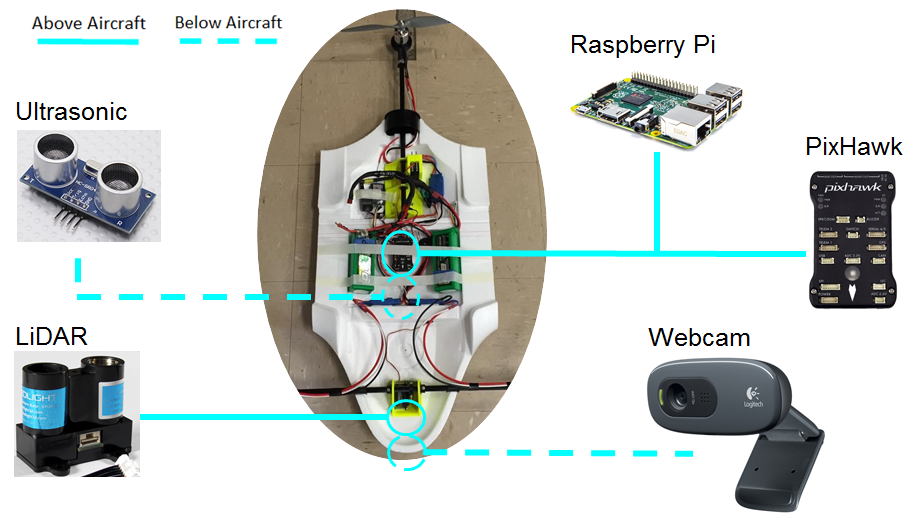
\includegraphics[width=300pt]{\IMAGEPATH /Diagrams/sensors}
	\caption{Onboard sensing capabilities, and mounting location, for Prototype \#2}
	\label{fig:sensing}
\end{figure}

\subsection{All Stages}

\subsubsection*{PixHawk Flight Controller}
As discussed previously, the PixHawk flight controller will control the aircraft's flight functionality, such as controlling motors and ailerons, and executing flight paths and commands.

\subsubsection*{Raspberry Pi}
The PixHawk is only capable of controlling the behaviour of the aircraft in response to input; to enable higher level behaviour, such as path planning and sensing, a separate microcontroller such as a Raspberry Pi is required. The Raspberry Pi will act as the aircraft's on-board computing platform, providing autonomy by giving flight commands to the flight controller, as well as the processing and intelligence for path planning and object detection. It will also retrieve flight data from the PixHawk and other sensors, and generate detailed flight logs for later review.

\subsection{Vertical Take-Off and Landing (M1)}
\subsubsection*{Ultrasonic Sensor}
The PixHawk comes equipped with a GPS module and altimeter, both of which can provide altitude measurements during flight. However, GPS is inherently inaccurate (up to $\pm$5m), and the performance of the altimeter depends heavily on environmental factors such as temperature. To augment these measurements, an ultrasonic sensor will be mounted underneath the aircraft. The ultrasonic sensor will be controlled by the Raspberry Pi, and will provide a more reliable and controllable height measurement during rotor-based flight, assisting with search and landing.

\subsection{Fixed-Wing Flight (M2)}
\subsubsection*{PixHawk Sensors}
During fixed-wing flight, it is imperative that the aircraft maintain a reliable measurement of its position to avoid the GeoFence boundaries specified in the Challenge. If at any point an aircraft breaches a boundary, it must immediately terminate its flight. In addition to the GPS and altimeter mentioned above, the PixHawk is also equipped with a 3-axis accelerometer and compass. Each of these sensors will enable the PixHawk to monitor the aircraft's position during flight.

\subsection{Aerial Search (M3)}
\subsubsection*{LiDAR}
During the aerial search stage the aircraft will be in low-altitude flight, putting it at risk of collision with trees, buildings, and other obstacles. To mitigate this risk, the aircraft will need to map the world around it to identify hazards. A LiDAR was chosen over a second ultrasonic sensor as it is capable of measuring larger distances, and with greater accuracy.\\

The LiDAR will be mounted in the nose of the aircraft. As it can only measure the range of objects directly in front of it, the LiDAR will be fixed to a system of two servos, as shown in Figure \ref{fig:lidar}, that will allow it to sweep a hemisphere in front of the aircraft. This will allow the generation of a 3D map of the environment around the aircraft, and will assist in path planning and obstacle avoidance.

\begin{figure}[!ht]
	\centering
	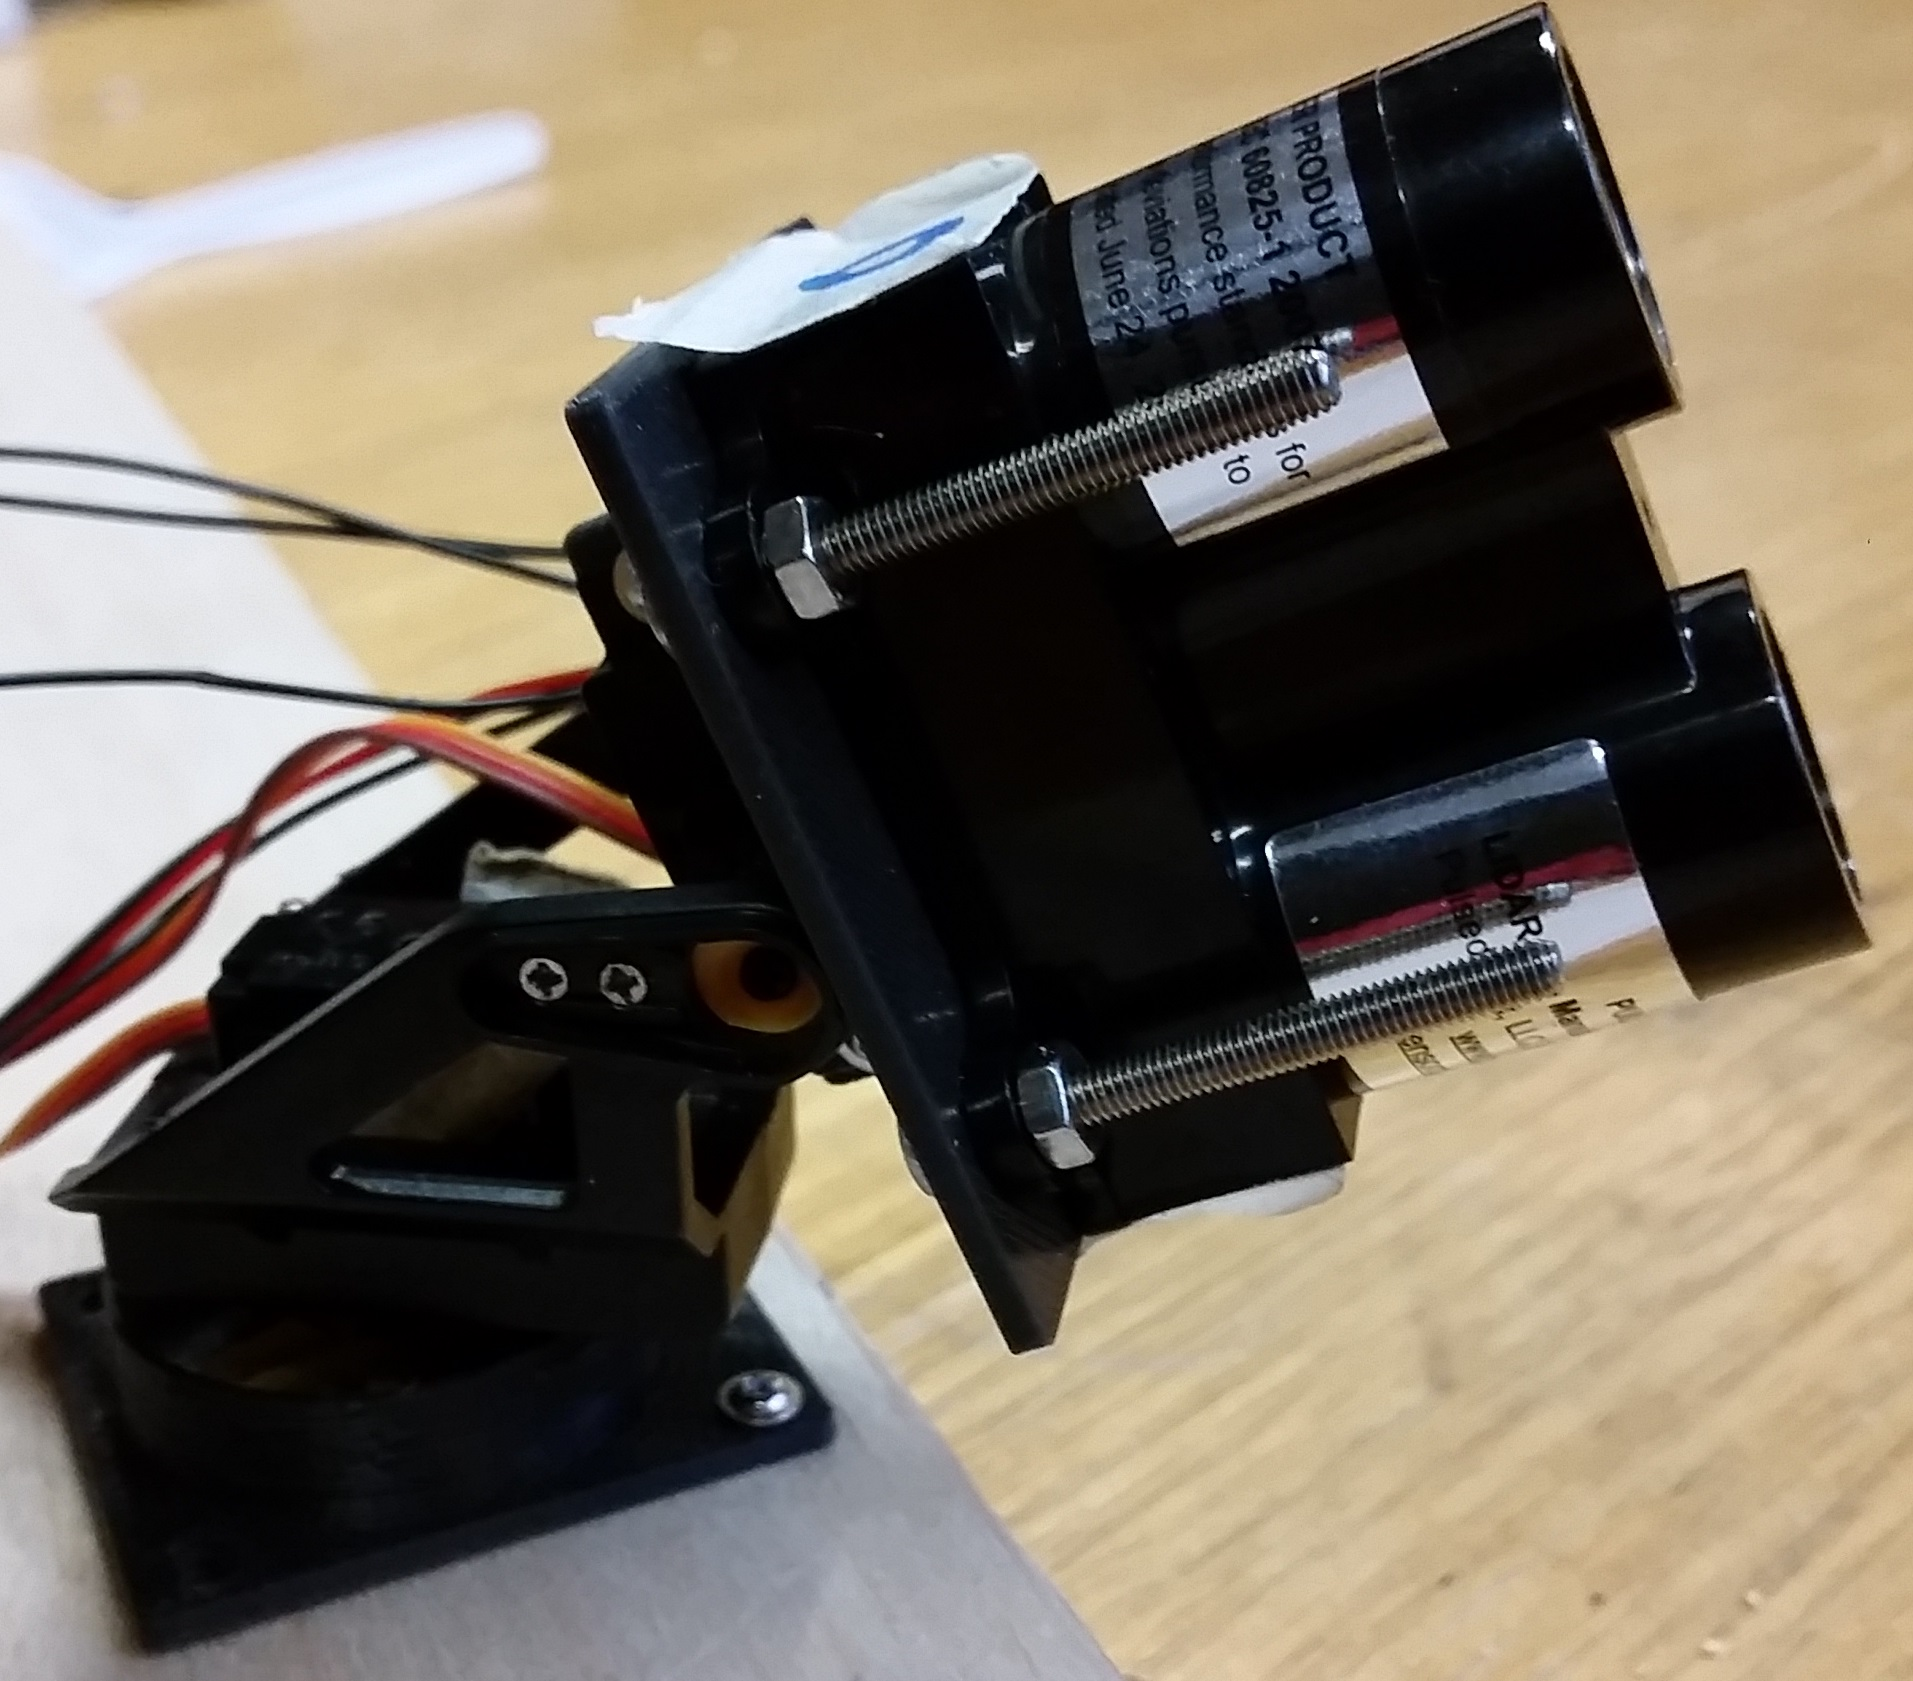
\includegraphics[width=100pt]{\IMAGEPATH /Prototype/lidar}
	\caption{LiDAR mounting}
	\label{fig:lidar}
\end{figure}

\subsubsection*{Webcam}
The only information provided to teams regarding Outback Joe is his love of Akubra hats and blue jeans. In order to detect Joe, the aircraft must be mounted with a visual sensor, such as a webcam. The webcam will be mounted beneath the nose of the aircraft, and will form the basis for identifying Joe using his hat and blue jeans, as well as providing real-time vision for the aircraft's obstacle avoidance maneuvers.

\subsection{Testing}
\subsubsection*{Ultrasonic and LiDAR}
To test the performance of the distance sensors, both sensors were placed in front of a series of obstacles at distances of 50cm, 1m and 5m, and 100 data points were collected at each distance. The sensors were able to measure distances within $\pm$10cm and $\pm$2cm for the ultrasonic and LiDAR respectively, but the performance of the LiDAR was noticeably better at measuring far away objects, as expected.  
	
\subsubsection*{GPS and Compass}  
During several flight tests it became evident that the data provided by the GPS and compass were wildly inaccurate, giving measurements that varied by up to $\pm$20m and $\pm$15$^\circ$ respectively. At any point during flight there may be up to 120A passing through the aircraft's internal circuitry, creating a large EM disturbance, in addition to the EM radiation from the other electronics. Given that both of these devices are susceptible to EM radiation \cite{ref:gpsinterference}, the module was mounted outside of the drone shell (as suggested by \cite{ref:gpsposition}), away from the electronics, resulting in the expected performance of $\pm$5m and $\pm$5$^\circ$ respectively.